\chapter{Methods}
\section{Part 1: Determination of electrode distance d}
\subsection{General approach}
The setup is illustrated in figure \ref{sec.setup_amp_1}. A cell surrounds the  epoxid resin sample and makes sure that the current flowing from the electrode to the wall is connected to the ground and does not count for the measurement. The DLPCA amplifier converts the measured current into a voltage and amplifies it. After a butterworth filter an ADC creates a signal that is processed with MATLAB. The butterworth filter ensures that frequencies above 100 kHz, which are not interesting for the mixed-frequency investigation, are cut out. 

\begin{figure}[htbp]
	\centering
	\includegraphics[width=\textwidth]{figures/Method/setup/setup_amplifier.png}		
	\caption[Kurze Abbildungsbeschreibung]{Setup for measurements\footnote{source: Raphael F\"arber}} 
	\label{sec.setup_amp_1}

\end{figure}
\label{sec:general_approach}
The following method is based on the assumption that  $\epsilon$ is always the same for the used samples when they are delivered. Thus, it is required to determine the distance of the electrodes for each delivered sample in order to be able to calculate the effective $\epsilon$ after below-PD current measurements, because the distance might vary considerably. 
At first, the initial $\epsilon_{eff}$ for two reference samples has to be obtained:\\
For the two reference samples the distance is measured optically with a microscope. By using the $d-C_0$-look-up table described in the following chapter the vacuum capacitance can be obtained from the optical distance measurement. Together with the measured capacitance $C*$ a guess of the effective epsilon for the used epoxy resin is possible. 

For forther samples, the capacitance $C*$ has to be measured. Together with the initial value of $\epsilon_{eff}$ of the reference samples one can obtain the vacuum capacitance $C_0$. By using the $d-C_0$ look up table a guess of the electrode distance d is possible. Now, the vacuum capacitance and the corresponding electrode distance are known for further measurements. Thus, it is possible to get the the values and changes in the effective permittivity with the calculated $C_0$.

\subsection{Simulation of vacuum capacitance} 
\label{sec.sim_vac_comsol}
As mentioned in the chapters before the vacuum capacitance cannot the calculated directly because of the complexity of the geometry. COMSOL is a simulation software that is suitable for a numerical estimation of permittivities or capacitances. The dependency of the vacuum capacity $C_0$ on the electrode distance d has to be simulated numerically both for the high-voltage setup and for the low-voltage setup. Although all measurements and the corresponding calculations in section \ref{sec:general_approach} can be carried out in the low-voltage setup it is handy to be able to do these calculations in the high-voltage setup as well. 


\begin{figure}[htbp]
	\centering
	\includegraphics{figures/COMSOL_Beispielbild.jpg}		
	\caption[Kurze Abbildungsbeschreibung]{E-Field simulation of the low-voltage test cell with cylindrically shaped electrodes(0.5 mm electrode distance)} \label{fig.comsol_beispiel}

\end{figure}
 
Figure \ref{fig.comsol_beispiel} shows the simulated field distribution in the low-voltage setup in COMSOL for an electrode with a cyclindrical geometry. Since the capacity of the setup and therefore also the currents are depending on the geometry of the electrode a conic electrode is simulated as well as shown in figure  \ref{fig.comsol_conic}

\begin{figure}[htbp]
	\centering
	\includegraphics[scale=0.3]{figures/Method/Part1_d_C0/conic.png}		
	\caption[Kurze Abbildungsbeschreibung]{E-Field simulation of the low-voltage test cell with conically shaped electrodes (0.5 mm electrode distance)} \label{fig.comsol_conic}

\end{figure}

In order to validate the simulations the capacitance of two spheres with a distance d are used as a reference. The following formula gives an approximation for the capacitance of two spheres with radius r and center distance d. \cite{Rawlins}
\begin{equation}
C=2 \pi \epsilon r ( ln 2 + \gamma -1/2 ln(2D-2)+O(2D-2))
\end{equation}
where D is the ratio of electrode distance over sphere diameter, i.e. $ D=\frac{d}{2r}$. As the electrodes have a spherical end with 8mm radius, the radius for the two capacitances is set 8mm as well. 
\begin{figure}[htbp]
	\centering
	\includegraphics[scale=0.3]{figures/Method/Part1_d_C0/sphere_capacity.jpg}		
	\caption[Kurze Abbildungsbeschreibung]{E-Field simulation of two spheres with 8mm radius } \label{fig.comsol_sphere}

\end{figure}

 There are several systematic errors that influence the vacuum capacity simulation. The inclined line on the right-hand side shows the air gap that is caused during the production process. This air gap between the wall of the low-voltage setup and the specimen causes an additional inhomogeneity. It is unavoidable in order to be able to remove the specimen from the pouring setup. This air gap should theoretically be 0.5 mm, but in practice it is expected to vary between 0 mm and 1 mm for the worst-case. The lookup table of d based on $C_0$ is based on an air gap of 0.5 mm, therefore the deviation from this value has to be investigated numerically.
Another systematic error is the deviation of the height of the specimen. During  the pouring process the height of the specimen cannot be fixed precisely. The maximum deviation is expected to be $\pm$ 0.5 mm. This deviation might occur during the production process of each new specimen. Thus, if the electrode distance of a specimen should be estimated by the method described these deviations can result in an error. 
 
\section{Suitability of current transformer for dielectric spectroscopy}
\subsection{The setup}
There are two general setups. One is the high-voltage setup and one the low voltage-setup. For testing the suitability of the current transformer the low voltage setup is sufficient except for the clamping test described in section \ref{clamping}. In order to get a similar current for the low-voltage setup as for the high-voltage setup a 1000 times higher vacuum capacitance is used in the Debye model. Therefore the selected vacuum capacitance is 3.3 nF whereas samples only have a vacuum capacitance of approximately 3.3 pF.  

The following graph \ref{sec.setup_amplifier} illustrates the setup for measurements without a current transformer. The DLPCA-200 is a variable gain low noise current amplifier that has a transimpedance gain between $10^3$ and $10^{11} V/A$. MATLAB automatically adapts its gain to a value that is suitable for the input voltage area of the ADC which is $\pm 10V$. 

\begin{figure}[htbp]
	\centering
	\includegraphics[width=\textwidth]{figures/Method/setup/setup_amplifier}		
	\caption[Kurze Abbildungsbeschreibung]{Setup for reference measurements {source: Raphael F\"arber, revised by authors}} 
	\label{sec.setup_amplifier}

\end{figure}

Afterwards, the DLPCA is replaced with a current transformer. 
\begin{figure}[htbp]
	\centering
	\includegraphics[width=\textwidth]{figures/Method/setup/setup_CTonly}		
	\caption[Kurze Abbildungsbeschreibung]{Setup for measurements with Current Transformer only {source: Raphael F\"arber, revised by authors}} 
	\label{sec.setup }

\end{figure}


\subsection{Signal analysis of the Debye model}

In order to emulate different dielectrica with their own respective dielectric loss tangent, different combinations of circuit elements were used.
Each different circuit accounts for another loss tangent with respect to frequency. With the objective to assess the performance of the current transformer, reasonably high values for the $tan\left(\delta\right)$ were assumed (i.e. 0.05 to 0.2) since a lower loss tangent
would require a higher resolution on the part of the current measurement. The vacuum capacitance was chosen to be about 1000 times larger than
the the one of the specimen for the purpose of generating the same magnitude of currents as in the high-voltage setup.
\begin{figure}
	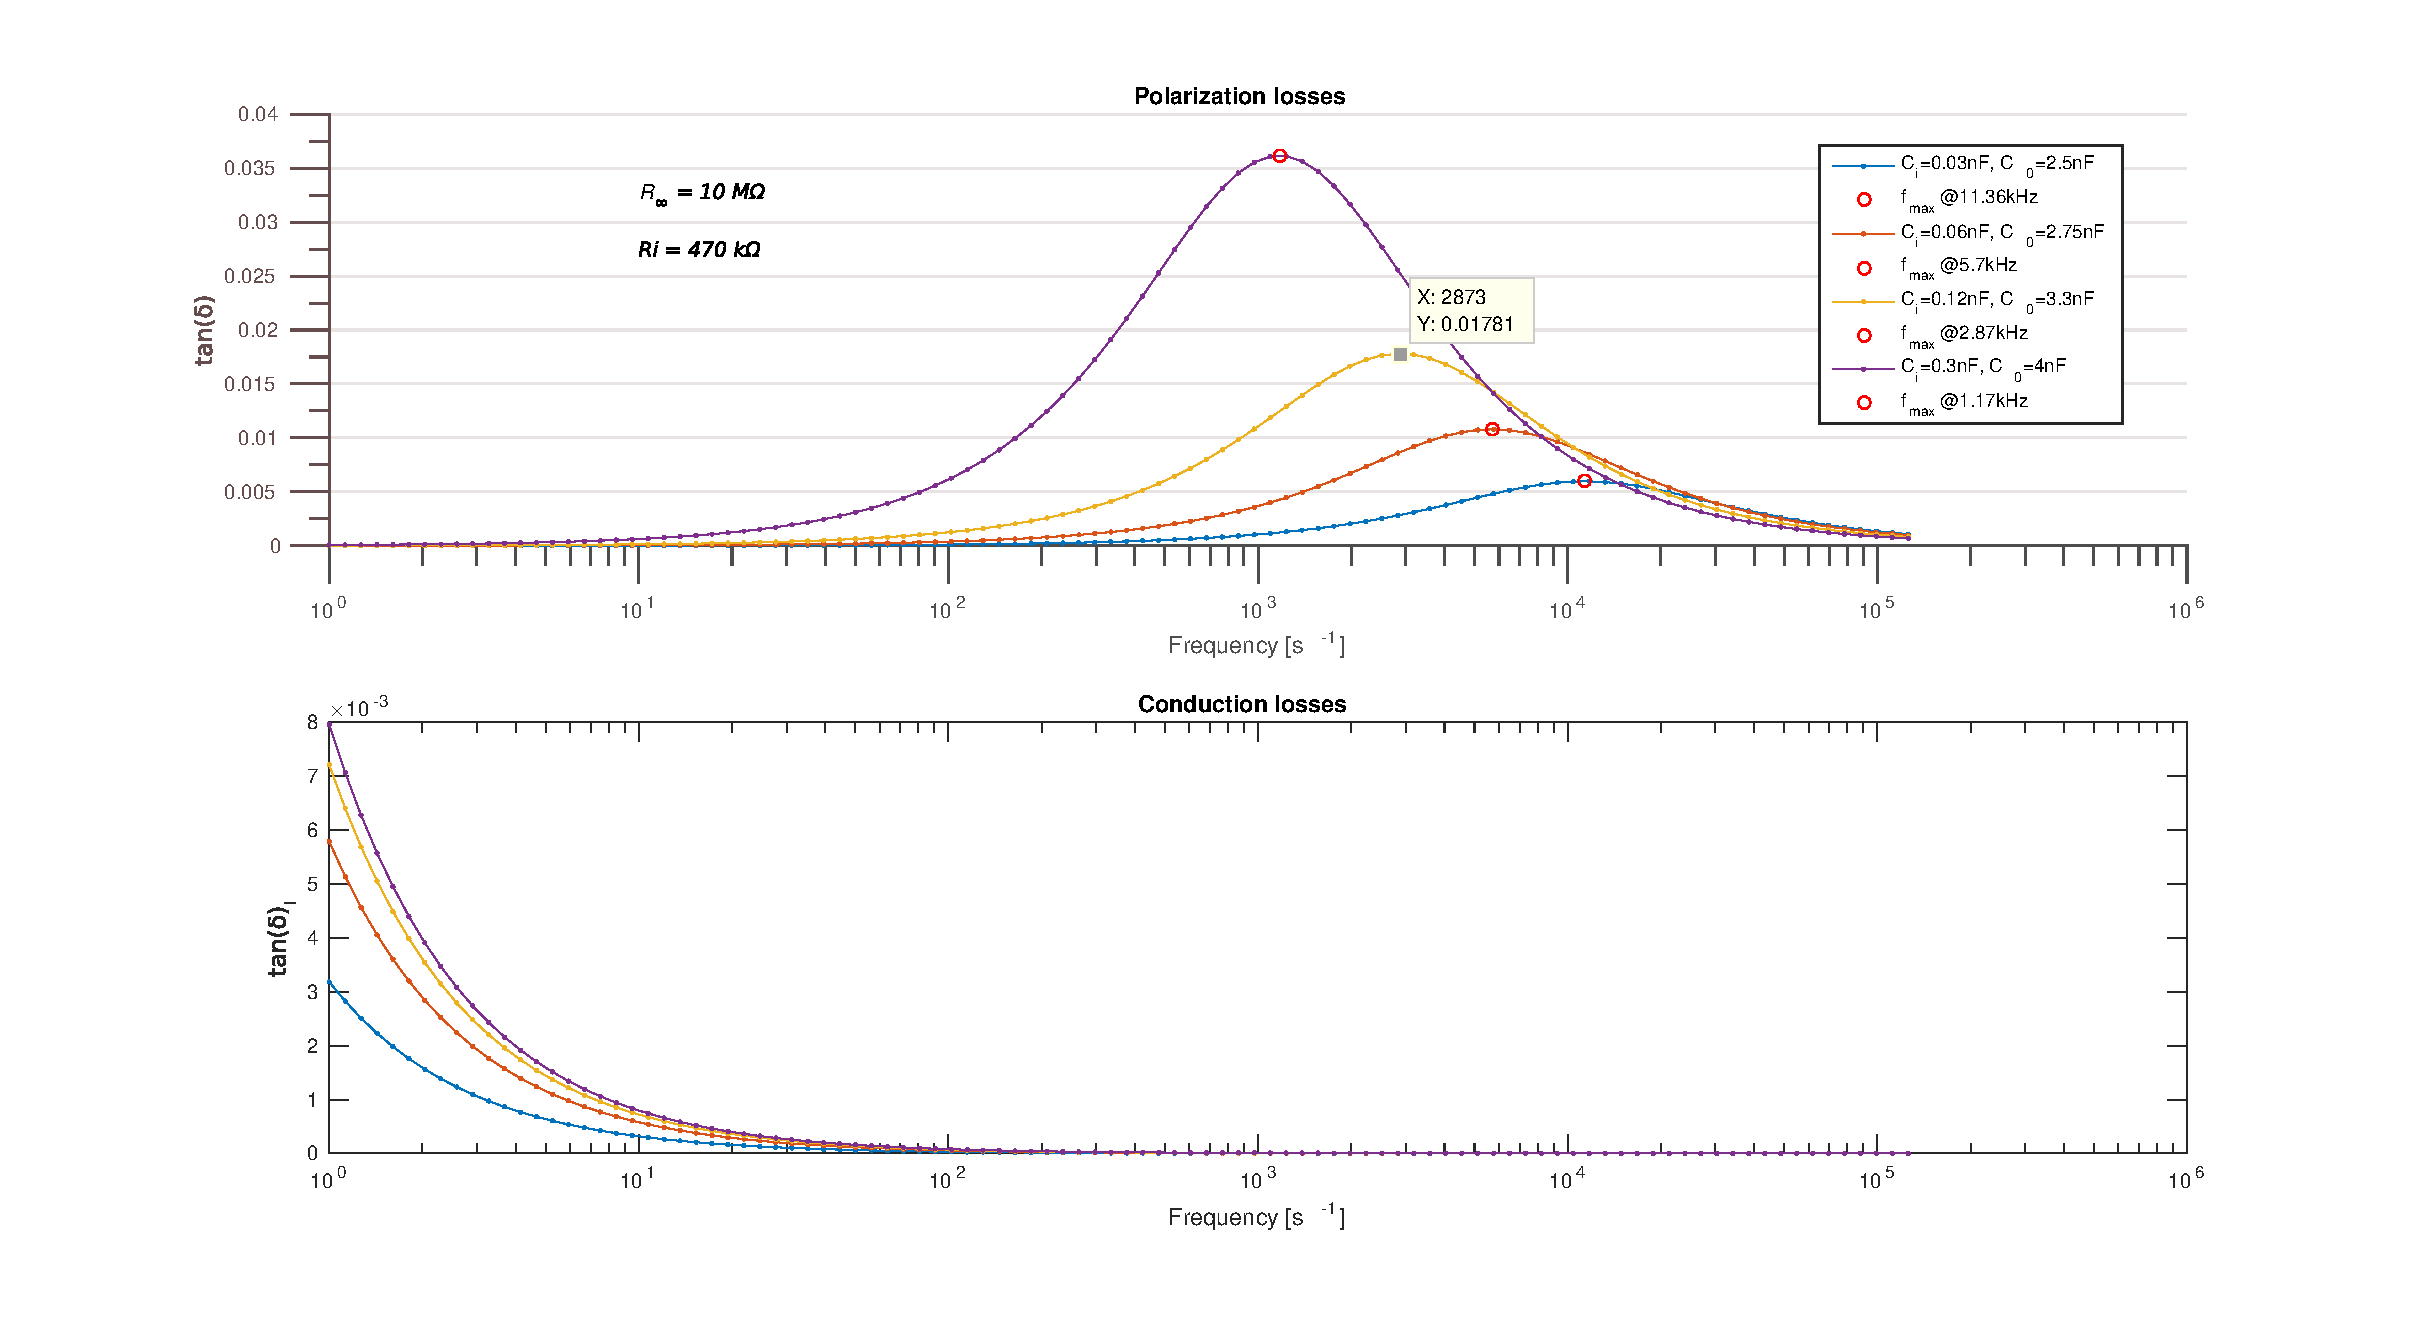
\includegraphics[width=\textwidth]{figures/Method/Dielectric_loss/polarizationmultiple.eps}	
	\caption{Polarization and Conduction losses for different frequencies and different parts in the Debye model}	
	\label{fig.debye-modell}
\end{figure}

In order to get a theoretical maximum tan($\delta$) of 0.0178 the parts shown in figure \ref{fig.debye-modell} are used. 
\begin{figure}
	\includegraphics[width=\textwidth]{figures/Method/debye-modell.jpg}	
	\caption{Debye model for max($tan(\delta)$)=0.0178 }	
	\label{fig.debye-modell}
\end{figure}

Once we insert the debye sample into the measurement setup of \ref{setup_amplifier} we can use the schematic in as a reference.

\begin{figure}
	\includegraphics[width=\textwidth]{figures/Method/debye-modell.jpg}	
	\caption{Debye model for max($tan(\delta)$)=0.0178 }	
	\label{fig.debye-modell}
\end{figure}

\subsection{Design of a holder for the Debye Equivalent Circuit}
For a lossy medium the Debye Network consists at least of a vacuum capacity $C_0$ and the term for the charging of the additional capacitance. The DC resistance has a very high value and might therefore be left out, i.e. $R_infty=infty$. Thus, it is reasonable to design a holder for the network that can hold three strands with two components each. Moreover, it has to fit into the low-voltage and high-voltage test cell, what specified the dimensions of the holder.  
Figure \ref{fig.CADgraph} shows the created holder which has a drawing that is depicted in figure \ref{fig.CADdrawing}.

\begin{figure}
\includegraphics[width=\textwidth]{figures/Method/CAD_MODEL/Gesamtanordnung.jpg}
\caption{CAD graph for the holder of the debye network. Created with SolidWorks Invetor}
\label{fig.CADgraph}
\end{figure}
\newpage

\begin{sidewaysfigure}
\includegraphics[width=0.99\textwidth]{figures/Gesamtanordnung.pdf}
    \caption{Drawing for the CAD holder}
    \label{fig.CADdrawing}
   \end{sidewaysfigure}	
\newpage
    

\subsection{Measurement of the textepsilon and the tan(textdelta) for the Debye model}

The aim is to have a current flwoing though the Debye model in the low-voltage setup that is of the same order as a current in the high voltage-setup. In order to have a comparable current for a voltage that is $1/1000$ of the high-voltage setup a capacitance $C_0$ for the Debye is selected 1000 times higher than the Capacitance of the samples. As the sample has a capacitance of 3.44 pF its equivalent $C_0$ in the debye-model is 3.3 nF. In order to get a tan($\delta$) of !!! $R_i$ is chosen as and $C_i$ is chosen as . This results in a loss 



\subsection{Integrator}
\subsection{Advantages of using an integrator}
As the used 16-bit DAC has a limited resolution it is advantageous to use an integrator in order to spread the frequencies of the signal over a larger timescale. This makes it possible to detect the different frequencies more accurately with the same DAC. 
A second reason to make use of an integrator is due to the fact that it adds an additional factor of $1/f$ to the Fourier spectrum of the output voltage signal. As the Fourier spectrum of the input signal is as well characterized by a $1/f$ decrease the integrator transforms the pulse signal back to a trapezoidal signal with a $1/f$-dependency in the Fourier spectrum. Since a $1/f$ dependency in the output signal is preferable to a constant Fourier spectrum due to better resolution for the first harmonic, the integrator improves the measurement as well. 

\subsection{Design of integrator}
The integrator should have two functions. On the hand side it should integrate signal on the other hand it should amplify the signal by a factor of 1000. This is due to the fact small below-PD-currents ($\sim$mA) should be measured. With a CT-sensitivity of $1V/A$ an amplification of 1000 is reasonable to use the range of measurable inputs of $\pm$ 10 V. These requirements can be achieved by a non-inverting integrator, which is shown in figure  \ref{fig.circuit}. 

\begin{figure}
\includegraphics[width=0.99\textwidth]{figures/Method/integrator/circuit.png}
    \caption{Property profile of the diverse library compared to the compound pool.}
    \label{fig.circuit}
    \end{figure}	


The integrator has the following transfer function: \\
\begin{equation}
	tf_{int}(j \omega)=\frac{1}{(1+s R_1 C_1)}\cdot(1+(\frac{1}/{R_2})\cdot(\frac{1}{R_3}+j \omega C_2)^{-1})
\end{equation}
The transfer function of the integrator is illustrated by the following bode plot. 

\begin{figure}

\includegraphics[width=\textwidth]{figures/Method/integrator/transferfunction_int.jpg}

\caption[Kurze Abbildungsbeschreibung]{Bode plot for the transfer function of an integrator } \ref{sec.Bodeplot}
\end{figure}

\begin{sidewaysfigure}
\includegraphics[width=0.99\textwidth]{figures/Method/integrator/PCB_Integrator.png}
    \caption{Printed Circuit Board Layout for the non-inverting ingrator with a DC voltage supply}
    
    \end{sidewaysfigure}	
    
    
    \newpage
    
    	\begin{sidewaysfigure}
\includegraphics[width=0.99\textwidth]{figures/Method/integrator/schematic.jpg}
 \caption{Property profile of the diverse library compared to the compound pool.}
  \end{sidewaysfigure}	

	



\subsection{Protective Clamping Capability of the current transformer}
\label{clamping}

